% This is based on the LLNCS.DEM the demonstration file of
% the LaTeX macro package from Springer-Verlag
% for Lecture Notes in Computer Science,
% version 2.4 for LaTeX2e as of 16. April 2010
%
% See http://www.springer.com/computer/lncs/lncs+authors?SGWID=0-40209-0-0-0
% for the full guidelines.
%
\documentclass{llncs}
\usepackage{setspace}
\usepackage{hyperref}
\usepackage{url}
\usepackage{listings}
\usepackage[pass]{geometry}
% \usepackage{vmargin}
\usepackage{fancyhdr}
\usepackage{amsmath}
\usepackage{amsfonts,amssymb,cite,float,graphicx}
% \usepackage[tight,footnotesize]{subfigure}
\usepackage[usenames]{color}
\usepackage{algorithm,algorithmic}
\usepackage{graphicx}
\usepackage{caption}
\usepackage{subcaption}
\usepackage{multicol}
\usepackage{float}
\usepackage{mathtools}

\doublespacing
\begin{document}

\title{Protecting Communications with Reinforcement Learning in a Multi-Agent Game}
%
\titlerunning{Hamiltonian Mechanics}  % abbreviated title (for running head)
%                                     also used for the TOC unless
%                                     \toctitle is used
%
\author{Faris Sbahi\inst{1} \and Barrett Ames\inst{2}}
%
\authorrunning{Faris Sbahi et al.} % abbreviated author list (for running head)
%
%%%% list of authors for the TOC (use if author list has to be modified)
%\tocauthor{Ivar Ekeland, Roger Temam, Jeffrey Dean, David Grove,
%Craig Chambers, Kim B. Bruce, and Elisa Bertino}
%
\institute{Primary\\
\email{faris.sbahi@duke.edu}
\and
Consultant\\
\email{barrett.ames@duke.edu}}

\maketitle              % typeset the title of the contribution

\begin{abstract}
Here we explore the ability of reinforcement learning (RL) agents to cooperate to establish a secure communication protocol in the face of an adversary without explicit communication. Hence, we construct a general sum mixed cooperative-competitive game to study the effectiveness of various multi-agent RL algorithms to perform in this environment. We compare our results with parallel experiments involving generative adversarial networks. We conclude that the Multi-Agent Deep Deterministic Policy Gradient algorithm prescribed in \cite{lowe2017multi} converges toward the desired behavior of securing protected communications in a period of time with which the other RL algorithms do not, and furthermore it represents a stronger result than the one involving GANs.
\keywords{reinforcement learning, multi-agent, communication, cryptography, generative adversarial networks, multi-agent actor-critic}
\end{abstract}
%
\section{Introduction}
%
%1. What problem does your project address? If you have chosen an application area, please remember that I may not be an expert in the application you have chosen, so be sure to describe the application area clearly.
%
%2. What methods did you use to address the problem?
%
%3. What is the reason you picked the methods you picked? Can you justify theoretically or empirically that this was the best choice?
%
%4. How did you validate your results?
%
%5. What difficulties did you encounter and how did you try to overcome them?
%
%6. What would be the next step if you were to extend this project?
%
%7. What did you learn from this?
%
%8. How did your consultant contribute to your project?
%
Reinforcement learning (RL) has been applied to increasingly complex tasks, ranging from Atari games to robotics. In most cases, the single-agent paradigm is pervasive given that predicting the behavior of other actors is unneeded.

Nevertheless, studying multi-agent systems is increasingly important if we expect to scale RL to interactive systems rather than applying the technique in a vacuum. We may expect that some sort of emergent, co-evolutionary behavior would evolve in a multi-agent setting. Hence, we can ask questions pertaining to social dilemmas\cite{leibo2017multi} and language\cite{foerster2016learning}, reaching Nash equilbria in cooperative or competitive games\cite{pinto2017robust}, or the ability to develop communication to achieve cooperative control tasks\cite{gupta2017cooperative} or even solve riddles\cite{foerster2016learning}.

Here we consider a mixed cooperative-competitive where an agent must communicate to another agent in the presence of an adversary. We find this worth considering because it allows us to study (1) the effectiveness of various RL and non-RL algorithms in a Markov game (defined below) of this type, (2) whether agents can protect their communications without being provided with an explicit cryptographic algorithm, and more broadly (3) whether and/or what kind of equilibria we observe depending on our algorithm and reward structures. 

Ultimately, we show that the simple multi-agent extensions of popular reinforcement learning algorithms perform poorly while the Multi-Agent Deep Deterministic Policy Gradient algorithm developed in \cite{lowe2017multi} produces a competitive game. Furthermore, the GAN context described in \cite{abadi2016learning} seems to allow for protected communications between agents but we'll argue that it's likely because of the limited decryption capability one might expect in this setup. 

Hence, the goal of this paper is to take the cryptography game defined in \cite{abadi2016learning} which is suitable for GANs, then to revise and modify it as a Markov game so it is suitable for the multi-agent RL context, and finally to evaluate the effectiveness of various MARL algorithms in this setting.
\subsection{The Problem}
%
The general game is simple.

We seek to define 3 agents Alice, Bob, and Eve such that Alice communicates a message to Bob who must reconstruct the message. Furthermore, adversary Eve observes the channel and additionally seeks to reconstruct the message. Hence, Alice and Bob should be penalized based off of Eve's reconstruction and rewarded based off of Bob's. Furthermore, Alice and Bob use a symmetric, randomly generated key (not available to Eve) to encode their message in a manner with which they define. 
\section{Methods}
\subsection{Markov Games}
First, we must extend the traditional Markov Decision Process (MDP) to the multi-agent setting. This is well documented and termed as a Markov Game\cite{leibo2017multi}. An $N$-agent Markov game is given by a collection states $\{ S \}$ with which any agent can take, in addition to actions $\{ A_1 \cdots A_N \}$ and observations $\{ O_1 \cdots O_N \}$. The $i$th agent uses a stochastic policy $\pi_i : O_i \times A_i \rightarrow [0,1]$ which takes the agent to the next state according to the state transition function $\mathcal{T}: S \times A_1 \times \cdots \times A_N \rightarrow S$. Similarly, the $i$th agent obtains rewards as a function of the state and action, and receives an observation. Each agent seeks to maximize its total expected return $R_i = \sum_{t=0}^T \gamma^t r_i^t$ where $r_i : S \times A_i \rightarrow \mathbb{R}$ is the reward associated with the taken action with $\gamma$ as the discount factor and $T$ the time horizon.  
%
\subsection{Extending Popular Single-Agent Algorithms}
With this notation in mind, we can readily popular single-agent algorithms to the multi-agent paradigm.

$Q$-learning uses an action-value function for a policy which can be written recursively as $Q^\pi(s,a)= \mathbb{E}_{s'}[r(s,a) + \gamma \mathbb{E}_{a'}[Q^\pi(s', a')]]$. Hence, $Q$-learning can be extended by simply allowing each agent to learn its independently optimal $Q_i$. 

Policy gradient 

\subsection{Multi-Agent Deep Deterministic Policy Gradient}

\section{Theoretical Matters}

\section{Experiments}

\subsection{GANs}

Following the experimental setup defined in \cite{abadi2016learning}, we setup a mirror experiment with code written in TensorFlow to observe whether neural networks can learn to protect communications between one another.

In summary, we had Alice, Bob, and Eve represented as neural networks. Alice has inputs $P$ and $K$ corresponding to the plaintext message and symmetric key and output $C$ the ciphertext. Bob has inputs $C$ and $K$ with output $P_B$ which is Bob's decryption of $P$. Finally, Eve simply has input $C$ and output $P_E$. 

Eve has the simple loss function which corresponds to the L1 distance between $P_E$ and $P$. Alice and Bob share the loss function which corresponds to L1 distance between $P_B$ and $P$ minus $(N/2 - \text{Eve L1 error})^2/(N/2)^2$ where $N$ is the length of $P$. The authors note the peculiarity of this loss function.

In addition to this peculiarity, the authors concede that they had to cute a number of corners to achieve the expected behavior. Note also that the agents are trained in an alternating pattern, switch back and forth between training Eve and then Alice and Bob together. Each epoch represents having trained both parties once. 

As in Figure 1, we found that the adversary quickly loses ability to decrypt and Alice and Bob converge to an effective protocol. Nevertheless, in all of our experimentations we found that once Eve drifted away from   
\begin{figure}
  \centering
    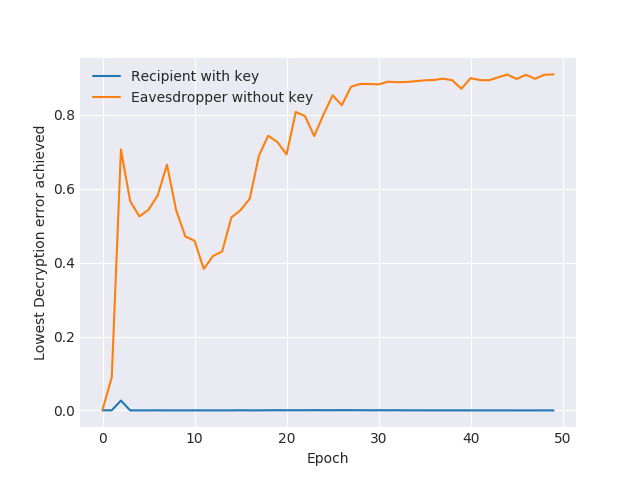
\includegraphics[width=\textwidth]{GAN_anc.png}
    \caption{Results observed using GANs}
\end{figure}

\subsection{DQN and Policy Gradient}

We omit any charts because we could not get either algorithm to converge to expected behavior in our experimentation given the number of episodes that time permitted. Nevertheless, this fits well with our theoretical considerations. We used an open source multi-agent reinforcement learning testbed (\url{https://github.com/sisl/MADRL}) to gather these results. 

\subsection{Multi-Agent Deep Deterministic Policy Gradient}

\subsection{Brief Comparison}

It's trivially difficult to make a direct comparison between the two set-ups because the games have a different fundamental structure. Nevertheless, we can still define our goal as to secure some means of private communication between agents in the face of an adversary with as little of 

\section{Conclusion}

We showed that it is difficult to derive meaningful results when using the classic RL algorithms in the multi-agent setting theoretically and empirically in the lens of protected communications. 

Nevertheless, interesting results are feasible with GANs though they might be weaker in nature than the results found using MADDPG given the weak ability of the adversary in the GAN context. 
\subsection{Further Development}

Other interesting multi-agent reinforcement learning algorithms exist and would be worth testing\cite{gupta2017cooperative}. Furthermore, we redefined the precise structure of our game several times during development, varying what types of actions each agent can make in addition to the reward structure. If time had allowed, it would've been useful to quantify the effect of these changes. It's also interesting to consider the case of having a greater number of adversaries or "good" communicators. 

Finally, there are several ways with which we could've empirically shown that GANs are weak at decrypting and hence don't represent a strong result in addition to the failure of traditional reinforcement learning algorithms in this arena. While we observed this qualitatively, it would be a sound extension to demonstrate this with further experiments. Potentially, too, it could be interesting to mix GANs with RL agents. 
\subsection{Thanks}

Thanks to Prof. Parr for giving me enough time to jam this project into a short period of time. I was able to learn how to run deep reinforcement learning experiments in the cloud, understand a bit about cryptography and GANs, develop an understanding of Markov games, multi-agent reinforcement learning, and some interesting algorithms that have been developed to fill the holes that I mentioned above in the simple single-agent extension algorithms. 

Thanks to Barrett for consulting on this project and being flexible with his schedule in addition to being happy to provide feedback. 

\bibliographystyle{ieeetr}
\bibliography{cs590}
\nocite{*}

%
% ---- Bibliography ----
%
%\begin{thebibliography}{5}
%
%\bibitem {clar:eke}
%Clarke, F., Ekeland, I.:
%Nonlinear oscillations and
%boundary-value problems for Hamiltonian systems.
%Arch. Rat. Mech. Anal. 78, 315--333 (1982)
%\end{thebibliography}
\end{document}
